\documentclass[a4 paper]{article}
\usepackage[T1]{fontenc}
\usepackage[utf8]{inputenc}
\usepackage[norsk]{babel}
\usepackage{amsmath}
\usepackage{amssymb}
\usepackage{hyperref}
\usepackage{parskip} %skip the indent of a new paragraph.
\usepackage{float}
\usepackage{graphicx}
\usepackage{listings}
\usepackage[per-mode=symbol]{siunitx}
\usepackage{epstopdf}
\usepackage[super]{nth}
\usepackage[toc,page]{appendix}
\usepackage{enumerate}
\usepackage{verbatim}
\usepackage[ruled, vlined, linesnumbered]{algorithm2e}
\usepackage{mathtools}
\usepackage{gensymb}
\usepackage{textcomp}
\usepackage{pdfpages}
%\lstset{language=Matlab, frame=single, breaklines=true,numbers=left, keywordstyle=\color{blue},rulecolor=\color{black},commentstyle=\color{gray}}

\usepackage{cleveref}
\usepackage[disable]{todonotes}

%% Brukes for tabeller (av likninger)
\usepackage{tabularx}
\def\tabularxcolumn#1{m{#1}}

\newcommand{\mbf}[1]{\mathbf[#1]}
\newcommand{\partialderiv}[2]{\frac{\partial{#1}}{\partial{#2}}} % prints partial derivative as a fraction

\DeclareUnicodeCharacter{2212}{-} % Needed to import matplolib figures without trouble

\renewcommand{\appendixname}{Vedlegg}

\begin{document}
    \title{Dokumentasjon TTK8}
    \author{Didrik Rokhaug}
    \maketitle

    \section{Sammendrag}
\todo[inline]{Skriv ett fornuftig sammendrag.}

I dette prosjektet er det blitt implementert en webserver som kna regulere mesking og gjæringsprossesen under ølbrygging. Systemet er implementert i programmeringspråket Rust og kjører på en Raspberry Pi. Det er laget for å kunne fungere med allerede eksisterende temperatursensorer og pådragsorganer. I tillegg til moduler for å bruke det eksisterende utstyret er det også blitt implementert en enkel simulator av meskingsprosessen for testing. Til tross for at systemet er komplekst, og har mange tråder har ett godt web-rammeverk og Rusts mekanismer for å hindre bugs gjort at implementasjonsarbeidet har vært nokså smertefritt. 
    \section{Innledning}
\todo[inline]{et kapittel som setter det du har gjort i en større sammenheng )hva inngår dette i, hilken funksjon har det du har laget. (IKKE LANGT)}

Når man brygger øl er det viktig å ha god konrtoll over temperaturen i prossessen. Dette gjelder både under meskingen og gjæringen. Det er derfor ønskelig å bruke en regulator for å styre temperaturen. Rusty Brew er en webserver som eksponerer ett API for automatisk regulering av prossesser der regulatoren skal følge en serie av referanser som er satt på forhånd. Samtidig er det mulig å hente ut gjeldende prossessparametre i sanntid, samt å hente ut logger i etterkant. Serveren er laget for å passe inn i ett eksisterende system, der alt av hardware for styring å måling av temperatur allerede er kjøpt inn. Det er derfor hovedsakelig ett software prosjekt, men valg av datamaskin er gjort for å kunne fungere med den eksisterende hardwaren.
    \section{Spesifikasjon og akseptansekriterier}
\todo[inline]{Punktvis funksjonell og theknidk dpesifikasjon og akseptansekriterier.}

Overordnede krav for systemet er at det skal kunne ta inn ett meske-forløp som det skal kunne regulere temperaturen etter, samt at det sakl kunne være mulig å følge med på prossessen i sanntid og hente ut en log etterpå.
Samtidig er det ønskelig at systemet skal fungere med allerede innkjøpte temperetursensorer av type DS18B20 og en kokeplate som kan styres med reléer. Temperatursensorene kommuniserer over en Onewire-buss. 

I tillegg til å kunne styre meskeprossessen er det en fordel å kunne styre temperaturen under gjæringsprossesen. Gjæringen foregår inni et kjøleskap, der kompressoren kan skrus av og på via ett relé. I tillegg er det ett varmeelement inni kjøleskapet som også kan styres via ett relé.

I tillegg skulle systemet implementeres i programmeringsspråket Rust for bedre sammspill med prosjektoppgaven.

Dette gir følgene overordnede krav til systemet:
\begin{itemize}
    \item Kunne regulere temperaturen i en prosses, via en gitt sensor og pådragsorgan.
    \item Kunne logge relevante prosess-variabler som målt temperatur og pådrag fra regulatoren.
    \item Gjøre det mulig for en klient  å hvise tilstanden i prosesses live.
\end{itemize}
    \section{Design}
\todo[inline]{Design, overordnet HW og/ellr SW (med begrunnete valg). Eventuell SW på blokknivå. Prøv å bruke navn som kan finnes igjen i vedlegget.}

Systemet er først og fremst ett software system, men med krav om at det skal kunne fungere med eksisterende hardware. Designet av systemet fokuserer derfor kunn på software-designet.

Systemet kan splittes opp i tre store moduler: interface, controller og log. Interface modulen er den som inneholder webserveren. 

\subsection{Log}
Designet av log-modulen er ganske enkelt, og vil i hovedsak dekkes sammen med implementasjonsdetaljene senere. Den ene store avgjørelsen som ble tatt på designet var hvordan loggene skulle lagres. De to alternativene var en database eller separate filer.
Fordelen med en database er at det er lett å søke etter datapunkter, og lett å legge til nye. Fordi en log er en sammenhengende serie oppføringer, og det eneste vi er interesert i er enten den siste oppføringen eller hele loggen ble det besluttet å bruker sepparate filer for hver log, og lagre den siste oppføringen i programmet for enkel tilgang.

\subsection{Controller}
Regulator-modulen ble designet med ett fokus på modularitet. Fordi systemet skal kunne brukes med flere typer pådragsorganer er sensorens og pådragorganets funksjonalitet abstrahert vekk bake ett trait\footnote{Rust sin versjon av abstrakt klasse}.

\subsection{Interface}
Interface modulen er den som implementerer eksponerer systemets funksjonalitet over internett. Her er det to ulike fremgangsmåter som ble vurdert. Den ene var å bruke en skytjeneste til å lagre data, og at systemet (som er koblet til hardware) bare sender statusoppdateringer til skytjenesten via MQTT. Denne fremgangsmåten kan også brukes uten en ekstern skytjeneste, men da legger man mer ansvar over på klienten. MQTT er en enkel publisher/subscriber protokol, og hadde hvert ganske lett å bruke, og man kan også bruke den som en requests/response protokoll. Hadde man brukt en skytjeneste kunne man brukt dens funksjoner for å lagre data, pluss at det finnes mange verktøy som er laget for å visualisere data fra skytjenester. Man hadde også sluppet å lage sin egen server-infrastruktur.

Det andre alternativet er å lage en egen HTTP server. Dette gjør at man også må lagre dataene selv, og sett opp det som trengs av infrastruktur for å håndtere flere requests samtidig. Å bruke HTTP gjør at klienten kan lages som en nettside, noe som gjør at klienten kan brukes på alle platformer med en nettleser. Samtidig er det også mulig å lage en vanlig skrivebordsklient. En ulempe med en requests/response protokoll vs en publisher/subscriber protokoll er at det ikke lenger er mulig å ``pushe'' oppdateringer til klienten. I stedet må klienten spørre hver gang den har lyst på ny data.

Beslutningen endte på HTTP. Denne avgjørelsen ble tatt av flere grunner. For det første blir det mulig med en web-klient, uten at man må bruke en skytjeneste (som koster penger), eller lage en sepparat server som kan oversette fra HTTP til MQTT. I tillegg har Rust flere rammeverk for implementering av webservere som jeg hadde lyst til å lære meg. Det er og lettere å bytte til en MQTT implementasjon enn det hadde vært å gå den andre veien.

Når besluttningen om å bruke HTTP var tatt var neste steg å bestemme seg for et API serveren skulle eksponere. API-et kan deles i to deler: log-delen og regulator-delen.
Logdelen av API-et er ganske enkelt\footnote{HTTP forespørslene er skrevet på følgenede måte: METODE sti/<variabel del av stien>}:
\begin{itemize}
    \item GET /logs, returnerer en liste over alle lagrede logger.
    \item GET /logs/<navn>, returnerer loggen med navn <navn>.
    \item DELTE /logs/<navn>, sletter loggen med navn <navn>.
\end{itemize}

For at brukeren skal slippe å måtte skrive inn det samme forløpet hver gang hvis han vil lage samme type øl igjen ble det bestemt at serveren skal kunne lagre referanse-serier. API-et for lagring å henting av referanseserier er veldig likt API-et for logger:
\begin{itemize}
    \item GET /reference\_series, returnerer en liste over alle lagrede referanseserier.
    \item GET /reference\_series/<navn>, returnerer referanseserien med navn <navn>.
    \item DELETE /reference\_series/<navn>, sletter loggen med navn <navn>.
    \item POST /reference\_series/<navn>, lagrer referanseserien med navn <navn>.
\end{itemize}

Fordi systemet skal være koblet til flere prosesser (mesking og gjæring) ble det bestemt å ha flere regulator-objekter, hver med sin egen innput utput og egene regulator-parametere. I interfacet blir ett slikt regulator-objekt kalt for en ``ressurs''. Hver ressurs lages ved oppstart av serveren, og hvilke ressurser som finnes er lagt inn i programmet. Klienten kan spesifisere hvilken ressurs den vil bruke ved å spesifisere navnet til ressursen. Dette gir det følgende API-et for å starte, og følge med på en prosess:
\begin{itemize}
    \item GET /resources, returnerer en liste over alle ressurser serveren har.
    \item GET /<ressurs>/values, returnerer de siste prosessverdiene hvis det er noen\footnote{Hvis ressursen regulerer en prosess vil den siste målte temperaturen, samt referanse og pådrag bli returnert. Hvis ressursen ikke er i bruk blir en feilmelding returnert.}.
    \item GET /start/<ressurs>/<profil>, ressurs <ressurs> starter å følge referanseserien <profil>.
\end{itemize}

Formatet på kommunikasjonen utover HTTP ble bestemt å være JSON, fordi de aller fleste språk har gode biblioteker for å lese dette formatet.

\begin{figure}
    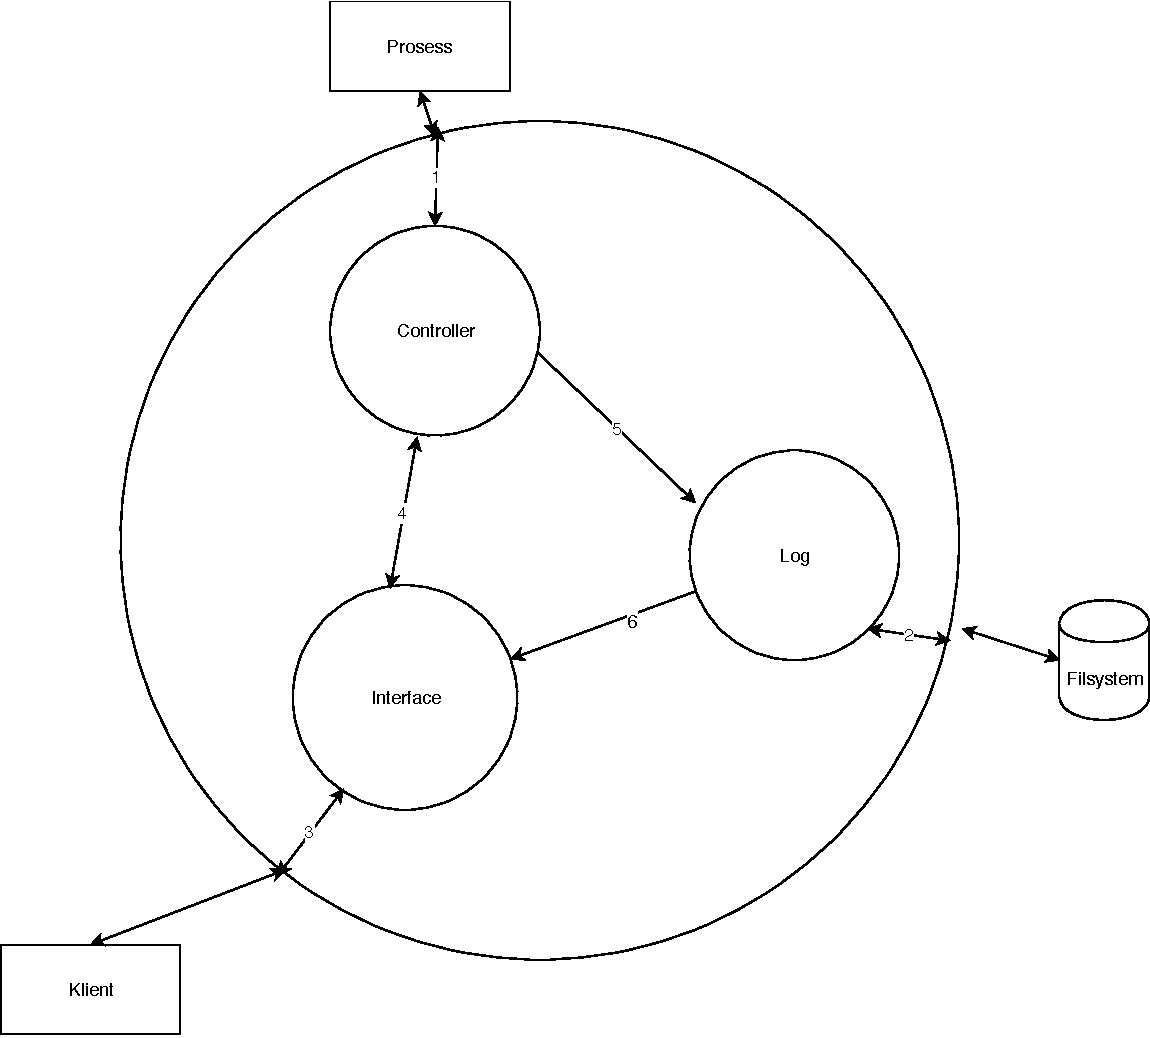
\includegraphics[width=\textwidth]{figures/system.pdf}
    \caption{Kontekstdiagram av hele systemet.}
    \label{fig:system}
\end{figure}

Totalt sett gir det ett design som ser ut som i figur \ref{fig:system}. Kommunikasjonen mellom modulene er følgende:
\begin{enumerate}
    \item Sensormålinger og pådrag.
    \item Lagring og lesing av logger og referanseserier.
    \item API-et beskrevet tidligere.
    \item Start av en prosess, lagring og lesing av referanseserier, og lesing av status på prosessen.
    \item Lagring av prosessverdier.
    \item Henting av logger.
\end{enumerate}


\begin{figure}
    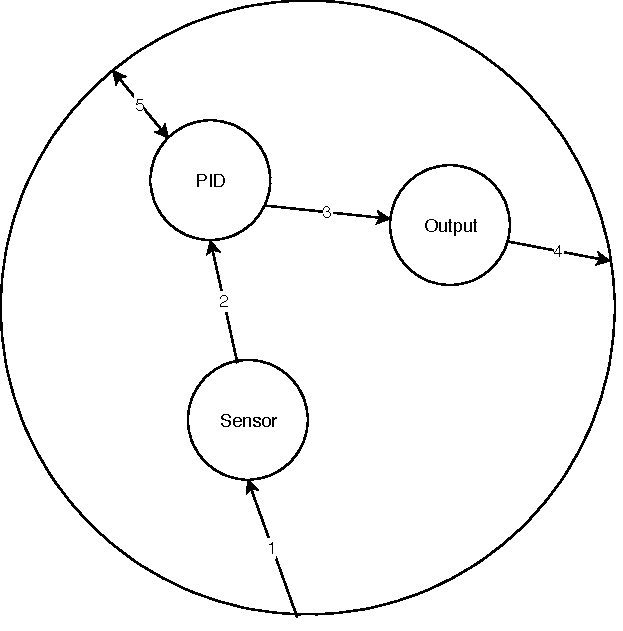
\includegraphics[width=\textwidth]{figures/controller.pdf}
    \caption{Kontekstdiagram for regulator-modulen.}
    \label{fig:regulator}
\end{figure}

Som nevnt er regulator-modulen den eneste som er litt komplisert designmessig. Sensor og Output modulene gir ett felles interface for ulike sensorer og pådragsorganer. PID modulen inneholder logikken til en PID-regulator. I tillegg har regulator-modulen en del logikk rundt oppstart og opprydning rundt prosessen. Hvordan modulen ser ut internt er vist i figur \ref{fig:regulator}, og kommunikasjonen knyttet til hver pil er listet opp nedenfor.
\begin{enumerate}
    \item Sensormålinger.
    \item Sensormålinger.
    \item Pådrag.
    \item Pådrag.
    \item Start av regulering, loggføring, lagring av referanseserier.
\end{enumerate}
    \section{Implementasjon}
\todo[inline]{Et kapittel med implementasjon, konkret hvordan er systemet laget med begrunnete valg. Forklar bruk av verktøy.}

Når det gjalt valg av maskinvare var det to muligheter. Den ene var å bruke en mikrokontroller for å lese fra sensorene, og styre pådragsorganene, og å ha en sepparat PC som kjørte serveren. Den andre var å gjøre alt fra en enkelt Raspberry Pi. Valget falt på å bruke Raspberry Pi, fordi man da slapp å jobbe med to ulike datamaskiner, det meste av utviklingen og testingen kunne skje på en hvilken som helst PC med Linux og i tillegg er Rust for embedded ikke veldig modent.

Når valet om å bruke filer for å lagre loggene var implementasjonen av log-modulen nokså enkel. Modulen har en datatype for en log, og en ``logger''. Loggerens oppgave er å abstrahere vekk den underliggende implementasjonen av log-systemet. Loggeren brukes mens loggen lages, i tillegg er det noen funksjoner som gir mulighet for å opperere på eksisterende logger.

Serveren ble implementert ved hjelp av rammeverket Rocket, ett av de største rammeverkene for webutvikling i Rust. Det bruker mye kodegenerering, og brukeren av rammeverket trenger i utgangspunktet bare å implementere funksjonene som kjøres når det kommer en forespørsel til en gitt sti. Ett annet alternativ er Iron, som er litt mindre, men det ble valgt vekk grunnet dårlig erfaring fra tidligere. Man kunne i tillegg ha lagd serveren selv ved hjelp av biblioteker, men det hadde blitt mye arbeid, for liten nytte. Rocket viste seg å være ganske lett å bruke. Det drar nytte av Rust sitt typesystem på en god måte, noe som gjør at brukeren av rammeverket bare trenger å si hvordan en type skal hentes ut fra en forespørsel, eller konverteres til en respons. Alt det andre av infrastruktur tar rammeverket seg av. På grunn av en antakelse om at Rocket hadde implementert en fornuftig måte å konvertere fra \texttt{std::io::Result}\footnote{Rust sin type for å håndtere mulige feil som har med fil-io å gjøre.} til \texttt{rocket::Response} ble det ikke implementert en egen \texttt{Result}-type. Under testingen viste det seg at dette fører til at brukeren bare får en HTTP-500 respons hvis noe går galt på serveren, selv om det ofte skyldes dårlig bruker-innput. Dette er en svakhet med den nåverende implementasjonen, fordi klienten ikke har noen mulighet til å si noe om hvorfor operasjonen feilet til sin bruker. Det er derimot ikke veldig vanskelig å endre dette i etterkant, men på grunn av andre prosjekter har denne forbedringen blitt prioritert ned. Rocket bruker naturlig nok mange tråder for å hpndtere ulike forespørsler, noe som fører til at objekter som kan brukes av flere forespørsler samtidig må være laget på en slik måte at de trygt kan deles mellom flere tråder. Dette la en del begrensninger på \texttt{Controller}-typen, som blir brukt både for å starte en ny prosess og å hente ut nåverende prosessverdier.

Ett stort problem her er at \texttt{Controller}-objekter inneholder objekter som implementerer \texttt{Input} og \texttt{Output}. Fordi man ikke vet hvilken type input og pådragsorgan man har må man bruke en form for generisk kode. Alle \texttt{Controller}-objektene legges i ett HashMap, og derfor må alle \texttt{Controller}-objektene ha samme type (og inneholde verdier av samme type). En mulig løsning er at \texttt{Controller}-objektene inneholder en referanse til innputt- og utputt-objektene. Her klager derimot Rust, fordi den ikke klarer å bevis at innputt- og utputt-objektene lever lenge nok. I tillegg må det være mulig å få tak i mutable referanser til utputt-objektet fra en annen tråd. Resultatet var å lagre en peker til ett heap-allokert objekt som må leve i hele programmets levetid, inni en atomisk referanse-tellende mutex. Dette sikrer den nødvendige synkroniseringen av tråder, samtidig som flere tråder får tilgang til objektet og de kan være sikre på at det ikke blir deallokert.

Den andre store utfordringen som ble møtt i løpet av implementeringen var hvordan infrastrukturen rundt selve reguleringen skulle være. Fordi API-et ikke kan blokkere er \texttt{start\_controlling} funksjonen nødt til å starte en ny tråd. Dette gjøres i \texttt{Controller}-objektets \texttt{start}-metode. Samtidig er det noe opprydning som må gjøres når prosessen er ferdig, og det hadde derfor vært ønskelig å vente helt til det skjer. Løsningen jeg endte opp med var å lage en tråd, som igjen lager de trådene som trengs for å faktisk gjøre reguleringen. Den første tråden venter så til de indre trådene er ferdige, før den gjør opprydningen, og selv gjør seg ferdig. For selve reguleringen blir det brukt tre tråder: en for å holde styr på hvor langt man har kommet i prosessforløpet, en som gjør selve reguleringen, og en som sørger for at de to andre trådene kjører med ett fast intervall. Disse tre trådene bruker kanaler for å kommunisere.

I tillegg til de to overnevnte utfordringene viste det seg å være mer problematisk å lese temperaturen fra temperatursensoren enn først antatt. I Rust finnes det ett maskinvare-uavhengig abstraksjonslag som gir tilgang til funksjonalitet som io-pinner og delays. Store deler av dette abstraksjonslaget er implementert for Linux, og det finnes ett bibliotek for den temperatursensoren som blir brukt i prosjektet som bruker dette abstraksjonslaget. Når dette biblioteket ble testet viste det seg derimot at det forsøkte å ``bit-bange'' onewire-protokollen. Dette viste seg å gå for tregt i en Linux user-space prosess til at det klarte å overholde timing-kravene til bussen. I stedet for dette biblioteket brukes derfor Linux sin kernel-modul for onewire. Denne modulen representerer hver sensor som en fil som man kan lese fra for å få den målte temperaturen.
    \section{Testing}
\todo[inline]{Et kapittel med uttesting mot funksjonell og teknisk spesifikasjon, hvordan virket systemet, forslag til eventuelle endringer}

Rust sitt typesystem er veldig kraftig, og kan forhidre mange vanlige bugs som ofte oppstår når man bruker pekere, i tillegg til å kunne forhidre data-races. Dette var til stor hjelp underveis i implementasjonen, da systemet inneholder flere tråder. I tillegg kan man bruke typesystemet til å bidra til å holde logikken og programflyten riktig ved å konstruere typene sine rett. Dette sørger for at man kan luke bort mange typer feil hvis programmet kompilerer. 

Testing ble ellers gjort ved å lage små programmer som gjorde en liten del av spesifikkasjonen. Ved å sjekke at disse programmene fungerte som de skulle kan man dermed være litt sikrere på at systemet fungerer som det skal.

Fordi systemet kjører på en Raspberry Pi kan alt untatt det som interfacer direkte med sensorer og pådragsorganer kjøre på en hvilken som helst datamaskin med Linux. Det ble derfor implementert ett simulert system, med simulert sensor og pådragsorgan slik at hele systemet kan testes på en vanlig datamaskin.

For å kunne teste serveren skikelig ble det også implementert ett klient-bibliotek i Python. Dette biblioteket ble så brukt i ett script som testet all funksjonaliteten til serveren ved vanlig bruk. Ved hjelp av dette scriptet ble det oppdaget at serveren ikke klarer å håndtere en forespørsel om å slette en logfil som er i bruk. Den ønskede oppførselen i dette tilfellet er å returnere en feil til klienten, men av en uviss grunn blir tråden som behandler forespørselen låst, og klienten får ingen respons på forespørselen. Hvorfor dette skjer er fortsatt uvisst, og må undersøkes nærmere.

I tillegg ble det i denne fasen oppdaget at ved de fleste feil i serveren får brukeren en HTTP 500 respons (intern server feil). Dette skjer selv om det er brukeren som er årsaken til at feilen skjer, og en feilkode i 400-familien skulle ha blitt returnert. Dette gjør at klienten ikke vet noe om grunnen til at forespørsel returente en feilmelding. Å endre dette er ikke veldig vanskelig, og fører ikke til store endringer i systemet, men har blitt prioritert ned i forhold til andre prosjekter for øyeblikket.
    \section{Konklusjon}
\todo[inline]{Finn en fornugtig måte å konkludere noe fornuftig.}

Selv om prosjektet i nåværende form oppfyller kravene er det flere ting som kan forbedres. Som nevnt får brukeren veldig lite informasjon om hvorfor en opperasjon gik galt. En annen ulempe med systemets nåværende implementasjon er at systemet ofte vil krasje, heller en å returnere en feilmelding. De fleste tilfellene dette skjer er steder der en feil i utgangspunktet ikke skal kunne skje, som for eksempel at man ikke kan lese en fil som man vet finnes. Det er heller ikke sannsynlig at hele systemet krasjer, på grunn av bruken av tråder og seppareringen av funksjonalitet. Denne mangelen kan rettes på omtrent samme måte som den første, men vil føre til større endringer. Derimot vil ikke disse endringene gjøre at eventuelle klienter må endres. Det eneste klientene vil se er at de får bedre feilmeldinger, og at de får flere av dem, i stedet for at serveren krasjer. 

Ett annet område systemet kan forbedres på er hva som skjer hvis serveren stopper å virke. Fordi den er koblet til ett fysisk sytem burde det helst ha vært noen mekanismer inne for automatisk restart og lignende, men dette er ikke implementert. Dette kan forsvares med at man har nok kontrol over systemet til at man kan forsikre seg om at dette nærmest aldri vil skje, men man kan aldri være helt sikre. En måte å forbedre denne situasjonen på ville vært å lage en watchdog som kan restarte serveren, og at serveren har en måte å se om den regulerte en prosess når den krasjet, for i så fall å fortsette der den slapp. 

Til tross for disse ulempene fungerer systemet som det skal, og på grunn av designet er det nokså robust mot feil. Dette skyldes også delvis Rust sine innebygde mekanismer for å forhindre bugs. 

    \appendix
    \section{Vedlegg}
\todo[inline]{Hvilke filer inneholder hvilke rutiner}

Serveren har følgende mappestruktur:
    \begin{itemize}
        \item Cargo.lock
        \item Cargo.toml
        \item build.rs
        \item src
        \begin{itemize}
            \item main.rs
            \item interface
            \begin{itemize}
                \item mod.rs
            \end{itemize}
            \item log
            \begin{itemize}
                \item mod.rs
            \end{itemize}
            \item controller
            \begin{itemize}
                \item mod.rs
                \item pid.rs
                \item mock.rs
                \item led.rs
                \item ds18b20.rs
                \item output
                \begin{itemize}
                    \item mod.rs
                \end{itemize}
                \item sensor
                \begin{itemize}
                    \item mod.rs
                \end{itemize}
            \end{itemize}
        \end{itemize}
    \end{itemize}

    I tilleg er api-client.py som inneholder kilent biblioteket i Python, og scriptet som ble brukt til testing. Det kan også produseres mer dokumentasjon fra koden ved å bruke cargo doc.

api-client.py inneholder Python klient biblioteket, og scriptet som er blitt brukt til testing.

I server-mappen finner vi koden til serveren. build.rs er ett program som kjøres når koden bygges som lager den mappestrukturen som serveren forventer. Cargo.toml inneholder en liste over biblioteker som blir brukt, mens Cargo.lock blir brukt av byggeverktøyet for å laste ned samme versjon som ble brukt under utviklingen av serveren. Selve kildekoden til serveren finnes i mappen src. main.rs inneholder main-funksjonen, som kjører når programmet blir kjørt. I tillegg inneholder den funksjoner som ble brukt under testing. De andre filene inneholder modulen med samme navn som filen. Filene som heter mod.rs inneholder modulen som har samme navn som mappen filen ligger i. For eksempel inneholder filen interface/mod.rs interface-modulen, som er der hvor selve serveren er implementert. led og ds18b20 inneholder moduler som interfacer med HW. mock har funksjonalitet for å simulere systemet. pid har selve regulator-logikken, mens controller har infrasturkturen rundt regulatoren.
\end{document}
